\chapter{Preliminaries}

\section{Linear Systems}
\subsection{Linear Time-Invariant Systems}\label{sec:linear_time_invariant_systems}
A discrete time state space representation of a linear dynamical system can be written as
\begin{subequations}\label{eq:2_lti}
\begin{equation}x(k+1) = Ax(k) + Bu(k)\end{equation}
\begin{equation}y(k) = Cx(k) + Du(k)\end{equation}
\end{subequations}
where $x(k) \in \mathbb{R}^n$ is a vector of the states of the system, $u(k) \in \mathbb{R}^m$ is a vector of input signals, and $y(k) \in \mathbb{R}^l$ is a vector of output signals for $k \in \mathbb{Z}$. $A$, $B$, $C$, and $D$ are the system matrices with dimensions $A\in\mathbb{R}^{n\times n}$, $B\in\mathbb{R}^{n\times m}$, $C\in\mathbb{R}^{l\times n}$, $D\in\mathbb{R}^{l\times m}$.
\begin{figure}[htb!]
	\centering
	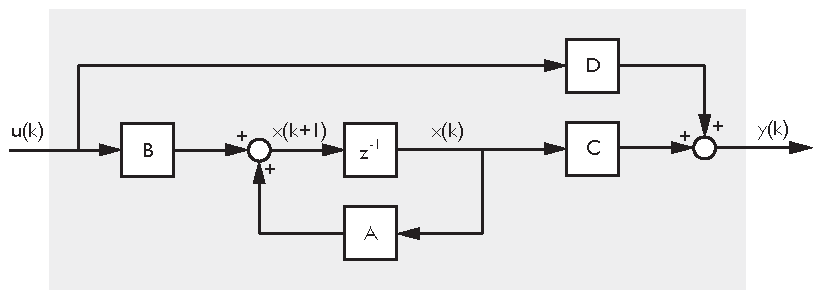
\includegraphics{../fig/lti_block_diagram.pdf}
	\caption{A block diagram of the state space representation of an LTI system.}
\end{figure}

It is important to see that the system state is not unique. That is, there are different state representations resulting in the same input-output behavior of the system. These differing states can be related by a similarity transform $T$ where $T$ is a real, nonsingular matrix:
\begin{equation*}
\tilde{x}(k) = T^{-1}x(k)
\end{equation*}
The state space representation of the system corresponding to the transformed state $\tilde{x}$ is given by
\begin{subequations}
\begin{equation*}\tilde{x}(k+1) = \tilde{A}\tilde{x}(k) + \tilde{B}u(k)\end{equation*}
\begin{equation*}y(k) = \tilde{C}\tilde{x}(k) + \tilde{D}u(k)\end{equation*}
\end{subequations}
with
\begin{equation*}
\tilde{A} = T^{-1}AT, \qquad
\tilde{B} = T^{-1}B, \qquad
\tilde{C} = CT, \qquad
\tilde{D} = D
\end{equation*}
As a result of this fact, we are able to extract the system matrices to within a similarity transform from input-output data through the application of subspace identification methods.

\subsection{Combined Deterministic-Stochastic LTI Systems}
Section \ref{sec:linear_time_invariant_systems} considered the case of a purely deterministic system; that is, a system operating in a noise-free environment. In practice, this rarely happens so we will now consider the case of the combined deterministic-stochastic LTI system operating in the presence of process and measurement noise. We append \ref{eq:2_lti} as follows
\begin{subequations}\label{eq:2_lti_noise}
\begin{equation}x(k+1) = Ax(k) + Bu(k) + w(k)\end{equation}
\begin{equation}y(k) = Cx(k) + Du(k) + v(k)\end{equation}
\end{subequations}
where $w(k)\in\mathbb{R}^1$ and $v(k)\in\mathbb{R}^1$ are the process and measurement noises, respectively. As is commonly done, we assume $w(k)$ and $v(k)$ are zero-mean white-noise sequences. 

If the system is observable, we can design a Kalman filter to estimate the system state \cite{kalman1960new}
\begin{equation*}
\hat{x}(k+1) = A\hat{x}(k) + Bu(k) + K\big(y(k) - C\hat{x}(k) - Du(k)\big)
\end{equation*}
where $K$ is the Kalman filter gain. If we denote 
\begin{equation*}
e(k) = y(k) - C\hat{x}(k) - Du(k)
\end{equation*}
to be the innovation sequence, we can rewrite the combined deterministic-stochastic system in Eq. (\ref{eq:2_lti_noise}) in the following equivalent \textit{innovation form}:
\begin{subequations}\label{eq:2_innovation}
\begin{equation}x(k+1) = Ax(k) + Bu(k) + Ke(k)\end{equation}
\begin{equation}y(k) = Cx(k) + Du(k) + e(k)\end{equation}
\end{subequations}
We will use the state space model in its innovation form to explain the subspace algorithm for identifying combined deterministic-stochastic LTI systems.


\section{Linear Algebra Tools}

\subsection{Hankel Matrices}
A Hankel matrix is a matrix $H \in \mathbb{R}^{m\times n}$ with constant skew-diagonals. In other words, the value of the $(i, j)^{\mbox{th}}$ entry of $H$ depends only on the sum $i + j$.
\begin{equation*}
H_{m,n} = \begin{bmatrix}
h_1 & h_2 & \cdots & h_n\\
h_2 & h_3 & \cdots & h_{n+1}\\
\vdots & \vdots & \ddots & \vdots\\
h_m & h_{m+1} & \cdots & h_{m+n-1}
\end{bmatrix}
\end{equation*}
If each entry in the matrix is also a matrix, it is called a block Hankel matrix.


\subsection{Fundamental Matrix Subspaces}
We require two of the fundamental matrix subspaces: the column space and the row space. The column space of a matrix $A \in \mathbb{R}^{m\times n}$ is the set of all linear combinations of the column vectors of $A$. The dimension of the column space is called the rank. The row space of a matrix $A \in \mathbb{R}^{m\times n}$ is the set of all linear combinations of the row vectors of $A$.


\subsection{Projections}


\subsection{Singular Value Decomposition}
Any matrix $A \in \mathbb{R}^{m\times n}$ can be decomposed by a singular value decomposition (SVD) given by
\begin{equation*}
A = U\Sigma V^T
\end{equation*}
where $U \in \mathbb{R}^{m\times m}$ and $V \in \mathbb{R}^{n\times n}$ are orthogonal matrices and $\Sigma \in \mathbb{R}^{m\times n}$ is diagonal matrix of the singular values $\sigma_i$ of $A$ ordered such that
\begin{equation*}
\sigma_1 \geq \sigma_2 \geq \cdots \geq \sigma_k > 0
\end{equation*}


\section{Quadrotor Rigid Body Dynamics}